\documentclass[tikz,border=3pt]{standalone}
\usepackage[utf8]{inputenc}
\usepackage[T1]{fontenc}
\usepackage{lmodern}
\renewcommand{\familydefault}{\sfdefault}
\usepackage{sansmath}\sansmath
\usepackage{pgfplots}\pgfplotsset{compat=1.18,/pgf/number format/use comma,/pgf/number format/1000 sep={.}}
\usetikzlibrary{arrows.meta,calc,positioning,decorations.pathmorphing,patterns}
% paleta del sitio
\definecolor{nar}{HTML}{E8680C}\definecolor{narc}{HTML}{FFB35C}\definecolor{hielo}{HTML}{FFF3E8}
\definecolor{tinta}{HTML}{1D1D1F}\definecolor{gris}{HTML}{6E6E73}\definecolor{lila}{HTML}{7C5CF0}
\definecolor{azul}{HTML}{2F6FD6}\definecolor{menta}{HTML}{17A673}\definecolor{coral}{HTML}{E8342A}
\begin{document}
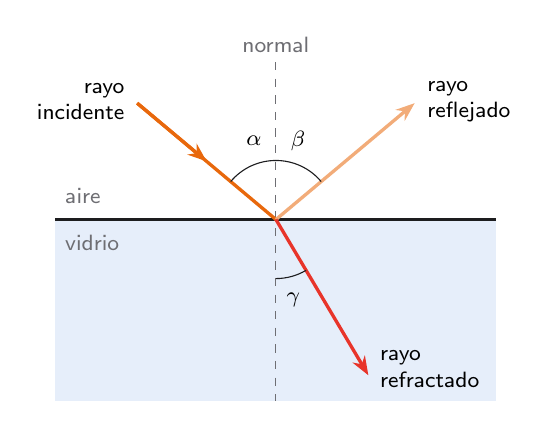
\begin{tikzpicture}[font=\footnotesize,>={Stealth[length=2.4mm]}]
\fill[azul!12] (-2.8,0) rectangle (2.8,-2.3);
\draw[thick,tinta] (-2.8,0) -- (2.8,0);
\node[right,text=gris] at (-2.8,0.3) {aire};
\node[right,text=gris] at (-2.8,-0.3) {vidrio};
\draw[gris,dashed] (0,2.0) -- (0,-2.3);
\node[gris,above] at (0,2.0) {normal};
\draw[very thick,nar] (-1.762,1.478) -- (0,0);
\draw[->,very thick,nar] (-1.762,1.478) -- (-0.88,0.739);
\draw[->,very thick,nar!55] (0,0) -- (1.762,1.478);
\draw[->,very thick,coral] (0,0) -- (1.174,-1.978);
\draw[tinta] (0,0.75) arc (90:140:0.75); \node at (-0.28,1.0) {$\alpha$};
\draw[tinta] (0,0.75) arc (90:40:0.75); \node at (0.28,1.0) {$\beta$};
\draw[tinta] (0,-0.75) arc (270:300.7:0.75); \node at (0.22,-1.02) {$\gamma$};
\node[left,align=right] at (-1.8,1.5) {rayo\\incidente};
\node[right,align=left] at (1.8,1.5) {rayo\\reflejado};
\node[right,align=left] at (1.2,-1.9) {rayo\\refractado};
\end{tikzpicture}
\end{document}
